\begin{enumerate}[(1)]
\item
	Transfer vertex capacities into edge capacities:
	\begin{itemize}
		\item Divide each vertex $u \in V$ into two vertexes, denoted by $u_{in}$ and $u_{out}$. Connect an edge from $u_{in}$ to $u_{out}$ with a capacity of $c$
		\item For each edge $\langle u, v \rangle \in E$, connect an edge from $u_{out}$ to $v_{in}$ with a capacity of $\infty$
		\item Calculate the maximum flow from $S_{in}$ to $T_{out}$
	\end{itemize}
	
	Transfer edge capacities into vertex capacities:
	\begin{itemize}
		\item For each vertex $u \in V$, still construct a vertex $v$ in $V'$ with a capacity of $\infty$
		\item For each edge $e\langle u, v, c\rangle \in E$, construct a vertex $p_e$ with a capacity of c, and connect edges from $u$ to $p_e$ and from $p_e$ to $v$
		\item Calculate the maximum flow from $S$ to $T$
	\end{itemize}
	\item Illustration
	
	The black edge's capacity is $\infty$, the red edge's capacity is $c$
	
	The black vertex's capacity is $\infty$, the red vertex's capacity is $c$
	
	These two pictures show Transfering vertex capacities into edge capacities. 
	\begin{figure}[!htbp]
		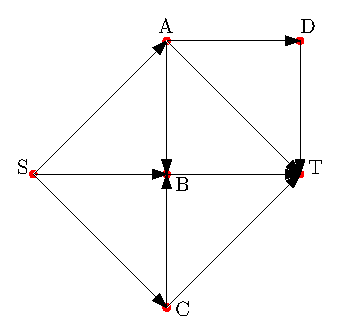
\includegraphics[totalheight=6cm]{source/xzj/pic1.eps}
		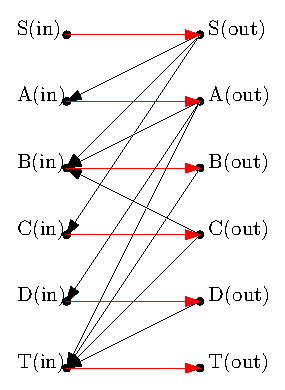
\includegraphics[totalheight=6cm]{source/xzj/pic2.eps}
	\end{figure}
	These two pictures show Transfering edge capacities into vertex capacities.
	\begin{figure}[!htbp]
		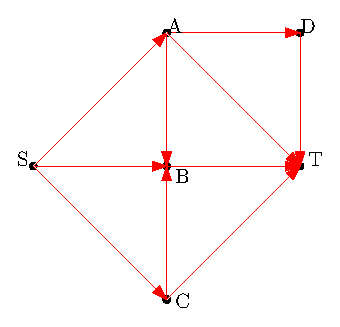
\includegraphics[totalheight=6cm]{source/xzj/pic3.eps}
		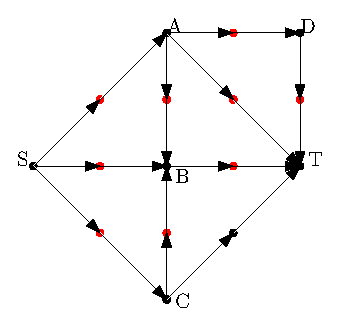
\includegraphics[totalheight=6cm]{source/xzj/pic4.eps}
	\end{figure}
	
	\item Construct a vertex capacities network $G = (V, E, c)$. The $c$ of $s$ and $t$ is $\infty$, and for other vertics, $c$ is $1$. 
	Calculate the maximum flow from $s$ to $t$.
	Each flow from $s$ to $t$ represent a path from $s$ to $t$. 
	Because the vertex capacities are 1 (except for $s, t$), these paths are internally vertex disjoint.
	There $k$ paths from $s$ to $t$, such that the paths are internally vertex disjoint if and only if the maximum flow if no less than $k$.
\end{enumerate}